\documentclass{article}
\usepackage{graphicx}
\usepackage{hyperref}
\usepackage{float}

\begin{document}

\title{A beginners guide to LaTeX}
\author{Lars H Lunde}
\date{\today\\v1.0}

\maketitle

\section{Intro}
Latex is an open source, cross platform document markup language. It is perfered by many academics because
of its maturity, the fact that it is open source, that it has a version for every operating system, including Haiku,
and that it has an advanced library for making and displaying mathematical equations.


\section{Starting using latex}
The first step of latex is downloading a LaTeX compiler for your chosen platform: \newline
\newline
\href{http://miktex.org/}{Windows: MikTex} \newline
\href{http://www.tug.org/mactex/}{Mac: MacTex} \newline
Linux: apt-get install texlive/pacman install texlive/emerge texlive \newline
(You will figure it out as you probably have chosen a distribution equal to your skill, and most distributions have TexLive in their repository)

\clearpage

\section{Markup}
\subsection{Header}
The general markup of LaTeX is starting with a header specifying documentclass, what packages to use, title, author, 
a command to make the title, a document begin tag and an end document tag: 


\begin{verbatim}
\documentclass{article}
\usepackage{graphicx}
\usepackage{hyperref}

\begin{document}

\title{A beginners guide to LaTeX}
\author{Lars H Lunde}
\date{\today\\v1.0}

\maketitle
\end{document}
\end{verbatim}

However for the purposes of simplicity I advice not using using packages that need custom package downloads. \bigskip
Everything in latex that is not plain text uses a tag \textbackslash markup. This much like learning code or how to
use linux requires mucking about with it and tweaking until you have a result that you find satisfying, and ask Google
PhD.

\section{Example section}
The format of the rest of the document is making sections.
\subsection{Subsection}
With sub sections
\subsubsection{Subsubsection}
and subsubsections


\begin{verbatim}

\section{Example section}
The format of the rest of the document is making sections.
\subsection{Subsection}
With sub sections
\subsubsection{Subsubsection}
and subsubsections

\end{verbatim}

All sections and subsections are automatically enumerated, however there is an override, specified in the 
"Tips and tricks section". 


\subsection{Markup}
Everything but plain text in latex start with a tag formatted using a backslash a codeword and a pair of curly brackets:

\begin{verbatim}
\end{verbatim}

\section{Pictures}
Adding pictures to a document is essential. Because of compatibility issues I highly encourage only using .png
files, and when putting them in to the document not to specify file ending, LaTeX does this automatically.
There are generally 2 ways of inputting pictures in to a LaTeX document.\newline
The easy way, which might require you to manipulate your pictures downward in size to fit the page.

\bigskip

\includegraphics{ubuntu}
\bigskip

\begin{verbatim}

\includegraphics{ubuntu}
\end{verbatim}

and the more customizable way:
\begin{verbatim}
\begin{figure}[p]
    \makebox[\linewidth]{
        
\includegraphics[width=1]{ubuntu}
    }
	\caption{Ubuntu logo}
\end{figure}
\end{verbatim}


\begin{figure}[p]
    \makebox[\linewidth]{
        
\includegraphics[width=1\linewidth]{ubuntu}
    }
	\caption{Ubuntu logo}
\end{figure}

\clearpage

However using the figure has way too many options for me to list, for further information read this article: \newline
\href{http://en.wikibooks.org/wiki/LaTeX/Floats,_Figures_and_Captions}{WikiBooks LaTeX: Floats Figures and Captions} \newline


\subsection{Reducing the margin}
In some cases the document can be too big for the document, and even though reducing margins is VERY frowned upon 
as it reduces printer compatibility, there is a way to do so in a pinch. As I will demonstrate with my shippo incredibly awful Shippo sudoku UML:
\clearpage

\begin{figure}[p]
    \vspace*{-4cm}
    \makebox[\linewidth]{
        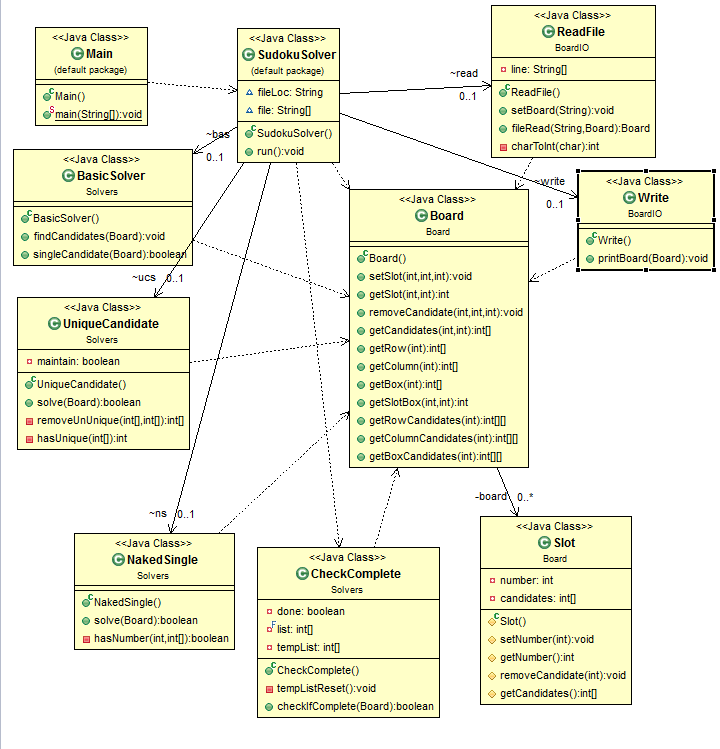
\includegraphics[width=1.5\linewidth]{uml}
    }
	\caption{UML Diagram}
\end{figure}

\clearpage

\begin{verbatim}
\begin{figure}[p]
    \vspace*{-4cm}
    \makebox[\linewidth]{
        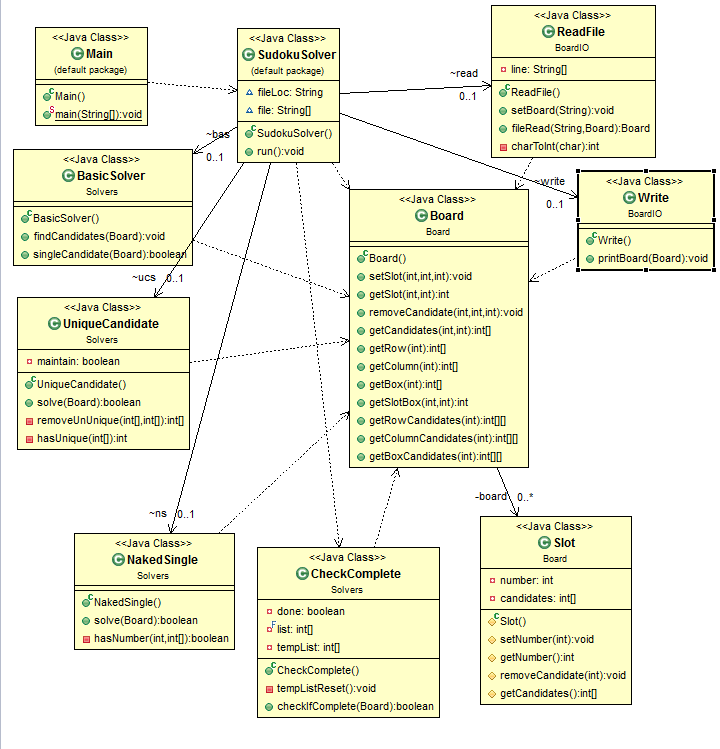
\includegraphics[width=1.5\linewidth]{uml}
    }
	\caption{UML Diagram}
\end{figure}
\end{verbatim}

\bigskip

The keyword being:
\begin{verbatim}
\vspace*{-4cm}
\end{verbatim}

\section{Tables}
Tables will be essential for making the test data documents, I reccomend using the template
I am using here, for more information go to \href{http://en.wikibooks.org/wiki/LaTeX/Tables}{Wiki Books LaTeX: Tables}.

\begin{flushleft}
\begin{tabular}{ | p{1cm} | p{1cm} | p{2.5cm} | p{2.5cm} | p{2.5cm} | p{2.5cm} |}
\hline
Test Red & Req being tested & Test Content & Input & Output & Pass Criteria \\ \hline
SE-F-001 & FR1 
& Check that system can store the first two days of the earliest permitted year 
& Enter 1st March 1971 at date prompt. Hit return, and enter 2nd March 1971 at date prompt  
& List of stored dates should now include those dates.& Data is stored correctly \\ \hline

\end{tabular}
\end{flushleft}

\bigskip
There is no denying this is a proper pain in the arse, but it has to be done.

\begin{verbatim}
\begin{flushleft}
\begin{tabular}{ | p{1cm} | p{1cm} | p{2.5cm} | p{2.5cm} | p{2.5cm} | p{2.5cm} |}
\hline
Test Red & Req being tested & Test Content & Input & Output & Pass Criteria \\ \hline
SE-F-001 & FR1 
& Check that system can store the first two days of the earliest permitted year 
& Enter 1st March 1971 at date prompt. Hit return, and enter 2nd March 1971 at date prompt  
& List of stored dates should now include those dates.& Data is stored correctly \\ \hline

\end{tabular}
\end{flushleft}
\end{verbatim}

\section{Writing code in to a LaTeX document}
Writing code in to a LaTeX document, or writing any text that contains markup signs must be
encapsulated in: \newline
\newline
\textbackslash begin\{verbatim\} \newline
Tags \newline
\textbackslash end\{verbatim\} \newline

And looks like this, this example is the FizzBuzz test written in LUA:

\begin{verbatim}
local boolean fb = true

for i = 1, 100 do
    if i % 3 == 0 then
        io.write("Fizz")
        fb = false
    end

    if i % 5 == 0 then
        io.write("Buzz")
        fb = false
    end

    if fb then
        io.write(i)
    end

    io.write("\n")
    fb = true
end
\end{verbatim}

As you can see it got printed out as is, with spaces and all the trimmings.
There are ways of making the code look more vibrant with plugins and special packages, for simplicity sake we will not be using those as recompiling 
the LaTeX on another machine can be tricky.
\clearpage

\section{Tips and Tricks, making LaTeX abide by your will}
\subsection{Pictures}
At times it seems that pictures in latex have a mind of their own, this is partially true,
it does what it finds best, but is in fact not sentient, there are 2 ways of forcing the picture in to place.
\bigskip
The first way is to make a include the: \newline
 \textbackslash usepackage\{float\} in the header and use the figure way of 
inputting a picture and using H as a parameter.

\begin{figure}[H]
    \makebox[\linewidth]{
        
\includegraphics[width=0.7\linewidth]{arch}
    }
\end{figure}
\bigskip

\begin{verbatim}
\begin{figure}[H]
    \makebox[\linewidth]{
        
\includegraphics[width=0.7\linewidth]{arch}
    }
\end{figure}
\end{verbatim}

However making some spacing around is always a good thing to do.
The command to do so is "\textbackslash bigskip", this will yield an empty line, whatever element comes before or after.
On the same note "\textbackslash newline" will clear the rest of the line and start a new one.

\bigskip

Another good trick in case you have a particularly big image is to use the "\textbackslash clearpage". 
This will start an entirely new page, and if you read the source of this document you will find it being used quite frequently.

\subsection{Disabling section enumeration}
Disabling section enumeration can be done by specifying: 
\begin{verbatim} 
\setcounter{secnumdepth\}{0}
\end{verbatim} 

\clearpage

\section{Useful links}
\href{http://tex.stackexchange.com/questions/41681/correct-way-to-bold-italicize-text}{Italisize and Bold} \newline
\href{http://anorien.csc.warwick.ac.uk/mirrors/CTAN/info/symbols/comprehensive/symbols-a4.pdf}{Special Characters and symbols in LaTeX}\newline
\href{http://en.wikibooks.org/wiki/LaTeX/List_Structures}{List Structures}\newline
\href{http://en.wikibooks.org/wiki/LaTeX/Tables}{Tables, especially for the test documents.}\newline




\end{document}